\PassOptionsToPackage{svgnames,dvipsnames,svgnames}{xcolor}
\newif\ifarxiv
\arxivfalse
\ifarxiv

%\documentclass[acmsmall,nonacm]{acmart}
\documentclass[acmsmall,screen,review,nonacm]{acmart}
\else
%%% Note: arxiv does not want line numbers (they are detected somehow, and are not allowed)
\documentclass[acmsmall,screen,review,nonacm]{acmart}
%\documentclass[acmsmall,nonacm]{acmart}
%\settopmatter{printfolios=false,printccs=false,printacmref=false}
% \settopmatter{printccs=false,printacmref=false}
\fi
  
%% For single-blind review submission
%\documentclass[acmlarge,review]{acmart}\settopmatter{printfolios=true}
%% For final camera-ready submission
%\documentclass[acmlarge]{acmart}\settopmatter{}

%% Note: Authors migrating a paper from PACMPL format to traditional
%% SIGPLAN proceedings format should change 'acmlarge' to
%% 'sigplan,10pt'.

% \bibliographystyle{ACM-Reference-Format}


%% Some recommended packages.
\usepackage{booktabs}   %% For formal tables:
                        %% http://ctan.org/pkg/booktabs
\usepackage{subcaption} %% For complex figures with subfigures/subcaptions
                        %% http://ctan.org/pkg/subcaption

\usepackage{graphicx}
%\usepackage{subfig}
%% Cyrus packages

\usepackage{multirow}
\usepackage{multicol}
\usepackage{microtype}
\usepackage{mdframed}
\usepackage{colortab}
\usepackage{mathpartir}
\usepackage{enumitem}
\usepackage{bbm}
\usepackage{stmaryrd}
\usepackage{mathtools}
\usepackage{leftidx}
\usepackage{todonotes}
\usepackage{xspace}
\usepackage{wrapfig}
\usepackage{extarrows}
\usepackage{listings}
% \usepackage[subtle]{savetrees}
\usepackage{listings}%
\lstloadlanguages{ML}
\lstset{tabsize=2, 
basicstyle=\footnotesize\ttfamily, 
% keywordstyle=\sffamily,
commentstyle=\itshape\ttfamily\color{gray}, 
stringstyle=\ttfamily\color{purple},
mathescape=false,escapechar=\#,
numbers=left, numberstyle=\scriptsize\color{gray}\ttfamily, language=ML, showspaces=false,showstringspaces=false,xleftmargin=15pt, 
morekeywords={string, float, int, bool},
classoffset=0,belowskip=\smallskipamount, aboveskip=\smallskipamount,
moredelim=**[is][\color{red}]{SSTR}{ESTR}
}

\lstdefinestyle{mystyle}{
otherkeywords = {match,Some,None,substitute,postpone,to, runtime,type, checking,unification, fails},
}

%"mystyle" code listing set
\lstset{style=mystyle}

%\usepackage[skip=2\baselineskip]{caption}
\usepackage{caption}
\newcommand{\li}[1]{\lstinline[basicstyle=\ttfamily\fontsize{9pt}{1em}\selectfont]{#1}}
\newcommand{\lismall}[1]{\lstinline[basicstyle=\ttfamily\fontsize{9pt}{1em}\selectfont]{#1}}

%% Joshua Dunfield macros
\def\OPTIONConf{1}%
\usepackage{joshuadunfield}

%% Can remove this eventually
\usepackage{blindtext}

\usepackage{enumitem}

%%%%%%%%%%%%%%%%%%%%%%%%%%%%%%%%%%%%%%%%%%%%%%%%%%%%%%%%%%%%%%%%%%%%%%%%%%%%%
%% Matt says: Cyrus, this package `adjustbox` seems directly related
%% to the `clipbox` error; To get rid of the error, I moved it last
%% (after other usepackages) and I added the line just above it, which
%% permits it to redefine `clipbox` (apparently also defined in
%% `pstricks`, and due to latex's complete lack of namespace
%% management, these would otherwise names clash).
\let\clipbox\relax
\usepackage[export]{adjustbox}% http://ctan.org/pkg/adjustbox
%%%%%%%%%%%%%%%%%%%%%%%%%%%%%%%%%%%%%%%%%%%%%%%%%%%%%%%%%%%%%%%%%%%%%%%%%%%%%%%%%


%%%%%%%%%%%%%%%%%%%%%%%%%%%%%%%%%%%%%%%%%%%%%%%%%%%%%%%%%%%%%%%%%%%%%%%%%%%%%%%%%
%\usepackage{draftwatermark}
%\SetWatermarkText{DRAFT}
%\SetWatermarkScale{1}
%%%%%%%%%%%%%%%%%%%%%%%%%%%%%%%%%%%%%%%%%%%%%%%%%%%%%%%%%%%%%%%%%%%%%%%%%%%%%%%%%


% A macro for the name of the system being described by ``this paper''
\newcommand{\HazelnutLive}{\textsf{Hazelnut Live}\xspace}
\newcommand{\Hazelnut}{\textsf{Hazelnut}\xspace}
% The mockup, work-in-progress system.
\newcommand{\Hazel}{\textsf{Hazel}\xspace}

% \newtheorem{theorem}{Theorem}[chapter]
% \newtheorem{lemma}[theorem]{Lemma}
% \newtheorem{corollary}[theorem]{Corollary}
% \newtheorem{definition}[theorem]{Definition}
% \newtheorem{assumption}[theorem]{Assumption}
% \newtheorem{condition}[theorem]{Condition}

\newtheoremstyle{slplain}% name
  {.15\baselineskip\@plus.1\baselineskip\@minus.1\baselineskip}% Space above
  {.15\baselineskip\@plus.1\baselineskip\@minus.1\baselineskip}% Space below
  {\slshape}% Body font
  {\parindent}%Indent amount (empty = no indent, \parindent = para indent)
  {\bfseries}%  Thm head font
  {.}%       Punctuation after thm head
  { }%      Space after thm head: " " = normal interword space;
        %       \newline = linebreak
  {}%       Thm head spec
\theoremstyle{slplain}
\newtheorem{thm}{Theorem}  % Numbered with the equation counter
\numberwithin{thm}{section}
\newtheorem{defn}[thm]{Definition}
\newtheorem{lem}[thm]{Lemma}
\newtheorem{prop}[thm]{Proposition}
\newtheorem{corol}[thm]{Corollary}
% \newtheorem{cor}[section]{Corollary}     
% \newtheorem{lem}[section]{Lemma}         
% \newtheorem{prop}[section]{Proposition}  

% \setlength{\abovedisplayskip}{0pt}
% \setlength{\belowdisplayskip}{0pt}
% \setlength{\abovedisplayshortskip}{0pt}
% \setlength{\belowdisplayshortskip}{0pt}



\makeatletter\if@ACM@journal\makeatother
%% Journal information (used by PACMPL format)
%% Supplied to authors by publisher for camera-ready submission
%\acmJournal{PACMPL}
%\acmVolume{1}
%\acmNumber{1}
%\acmArticle{1}
%\acmYear{2018}
%\acmMonth{3}
%\acmDOI{10.1145/nnnnnnn.nnnnnnn}
%\startPage{1}
\else\makeatother
%% Conference information (used by SIGPLAN proceedings format)
%% Supplied to authors by publisher for camera-ready submission
% \acmConference[]{ACM SIGPLAN Conference on Programming Languages}{January 01--03, 2017}{New York, NY, USA}

%\acmYear{2018}
%\acmISBN{978-x-xxxx-xxxx-x/YY/MM}
%\acmDOI{10.1145/nnnnnnn.nnnnnnn}
%\startPage{1}
\fi


%% Copyright information
%% Supplied to authors (based on authors' rights management selection;
%% see authors.acm.org) by publisher for camera-ready submission
\setcopyright{none}             %% For review submission
%\setcopyright{acmcopyright}
%\setcopyright{acmlicensed}
%\setcopyright{rightsretained}
%\copyrightyear{2017}           %% If different from \acmYear


% \fancyfoot{} % suppresses the footer (also need \thispagestyle{empty} after \maketitle below)


%% Bibliography style
\bibliographystyle{ACM-Reference-Format}
%\bibliographystyle{abbrvnat}
%% Citation style
%% Note: author/year citations are required for papers published as an
%% issue of PACMPL.
\citestyle{acmauthoryear}   %% For author/year citations

% !TEX root = ./type-inference-paper.tex

\newcommand{\mynote}[3]{\textcolor{#3}{\textsf{{#2}}}}
\newcommand{\rkc}[1]{\mynote{rkc}{#1}{blue}}
\newcommand{\cy}[1]{\mynote{cy}{#1}{purple}}
\newcommand{\mah}[1]{\mynote{cy}{#1}{green}}
\newcommand{\matt}[1]{{\color{blue}{\textit{Matt:~#1}}}}

\newcommand{\cvert}{{\,{\vert}\,}}

%% https://tex.stackexchange.com/questions/9796/how-to-add-todo-notes
\newcommand{\rkcTodo}[1]{\todo[linecolor=blue,backgroundcolor=blue!25,bordercolor=blue]{#1}}

\newcommand{\mattTodo}[1]{\todo[linecolor=green,backgroundcolor=green!2,bordercolor=green]{\tiny\textit{#1}}}
\newcommand{\mattOmit}[1]{\colorbox{yellow}{(Matt omitted stuff here)}}

\def\parahead#1{\paragraph{\textbf{#1.}}}
%% \def\paraheadNoDot#1{\paragraph{{\textbf{#1}}}}
\def\subparahead#1{\paragraph{\textit{#1.}}}
%% \def\paraheadindent#1{\paragraph{}\textit{#1.}}
%% \def\paraheadindentnodot#1{\paragraph{}\textit{#1}}

% \newcommand{\ie}{{\emph{i.e.}}}
% \newcommand{\eg}{{\emph{e.g.}}}
% \newcommand{\etc}{{\emph{etc.}}}
% \newcommand{\cf}{{\emph{cf.}}}
% \newcommand{\etal}{{\emph{et al.}}}

%% \newcommand{\hazel}{\ensuremath{\textsc{Hazel}}}
%% \newcommand{\sns}{\ensuremath{\textsc{Sketch-n-Sketch}}}
%% \newcommand{\deuce}{\ensuremath{\textsc{Deuce}}}
\newcommand{\Elm}{\ensuremath{\textsf{Elm}}}
\newcommand{\sns}{\ensuremath{\textrm{Sketch-n-Sketch}}}
\newcommand{\deuce}{\ensuremath{\textrm{Deuce}}}

\newcommand{\sectionDescription}[1]{\section{#1}}
\newcommand{\subsectionDescription}[1]{\subsection{#1}}
\newcommand{\subsubsectionDescription}[1]{\subsubsection{#1}}
%% \newcommand{\subsectionDescription}[1]{\subsection*{#1}}
\newcommand{\suppMaterials}{the Supplementary Materials}

\newcommand{\defeq}{\overset{\textrm{def}}{=}}

\newcommand{\eap}{action suggestion panel\xspace}
\newcommand{\Eap}{Action suggestion panel\xspace}

\newcommand{\myfootnote}[1]{\footnote{ #1}}

\def\sectionautorefname{Section}
\def\subsectionautorefname{Section}
\def\subsubsectionautorefname{Section}

\newcommand{\code}[1]{\lstinline{#1}}

% Make italic?
%\newcommand{\Property}[1]{\emph{#1}}
\newcommand{\Property}[1]{\textrm{#1}}

% Calling out Cyrus's favorite verb, 'to be' ;)
\newcommand{\IS}{\colorbox{red}{is}\xspace}

\newcommand{\codeSize}
  %% {\footnotesize}
  {\small}

%\newcommand{\JoinTypes}[2]{\textsf{join}~~#1~~#2}
\newcommand{\JoinTypes}[2]{\textsf{join}(#1,#2)}

%%%%%%%%%%%%%%%%%%%%%%%%%%%%%%%%%%%%%%%%%%%%%%%%%%%%%%%%%%%%%%%%%%%%%%%%%%%%%%%%
%% Spacing

\newcommand{\sep}{\hspace{0.06in}}
\newcommand{\sepPremise}{\hspace{0.20in}}
\newcommand{\hsepRule}{\hspace{0.20in}}
\newcommand{\vsepRuleHeight}{0.08in}
\newcommand{\vsepRule}{\vspace{\vsepRuleHeight}}
\newcommand{\miniSepOne}{\hspace{0.01in}}
\newcommand{\miniSepTwo}{\hspace{0.02in}}
\newcommand{\miniSepThree}{\hspace{0.03in}}
\newcommand{\miniSepFour}{\hspace{0.04in}}
\newcommand{\miniSepFive}{\hspace{0.05in}}

%%%%%%%%%%%%%%%%%%%%%%%%%%%%%%%%%%%%%%%%%%%%%%%%%%%%%%%%%%%%%%%%%%%%%%%%%%%%%%%%

% \lstset{
% %mathescape=true,basicstyle=\fontsize{8}{9}\ttfamily,
% literate={=>}{$\Rightarrow$}2
%          {<=}{$\leq$}2
%          {->}{${\rightarrow}$}1
%          {\\\\=}{\color{red}{$\lambda$}}2
%          {\\\\}{$\lambda$}2
%          {**}{$\times$}2
%          {*.}{${\color{blue}{\texttt{*.}}}$}2
%          {+.}{${\color{blue}{\texttt{+.}}}$}2
%          {<}{${\color{green}{\lhd}}$}1
%          {>?}{${\color{green}{\rhd}}$?}2
%          {<<}{${\color{green}{\blacktriangleleft}}$}1
%          {>>?}{${\color{green}{\blacktriangleright}}$?}2
%          {\{}{${\color{blue}{\{}}$}1
%          {\}}{${\color{blue}{\}}}$}1
%          {[}{${\color{purple}{[}}$}1
%          {]}{${\color{purple}{]}}$}1
%          {(}{${\color{darkgray}{\texttt{(}}}$}1
%          {)}{${\color{darkgray}{\texttt{)}}}$}1
%          {]]}{${\color{gray}{\big(}}$}1
%          {]]}{${\color{gray}{\big)}}$}1
% }

% !TEX root = ./type-inference-paper.tex

% reverse Vdash


% Violet hotdogs; highlight color helps distinguish them
\newcommand{\llparenthesiscolor}{\textcolor{violet}{\llparenthesis}}
\newcommand{\rrparenthesiscolor}{\textcolor{violet}{\rrparenthesis}}

% HTyp and HExp
\newcommand{\hcomplete}[1]{#1~\mathsf{complete}}

% HTyp
\newcommand{\htau}{\dot{\tau}}

\newcommand{\tarrnp}[2]{#1 \rightarrow #2}
\newcommand{\trul}[2]{\inparens{#1 \Rightarrow #2}}
\newcommand{\trulnp}[2]{#1 \Rightarrow #2}
\newcommand{\tnum}{\mathtt{num}}
\newcommand{\tehole}{\llparenthesiscolor\rrparenthesiscolor}
\newcommand{\tsum}[2]{\inparens{{#1} + {#2}}}
\newcommand{\tprod}[2]{\inparens{{#1} \times {#2}}}
\newcommand{\tunit}{\mathtt{1}}
\newcommand{\tvoid}{\mathtt{0}}

\newcommand{\tcompat}[2]{#1 \sim #2}
\newcommand{\tincompat}[2]{#1 \nsim #2}

% HExp
\newcommand{\hexp}{\dot{e}}
\newcommand{\hlam}[3]{\inparens{\lambda #1:#2.#3}}
\newcommand{\hap}[2]{#1(#2)}
\newcommand{\hapP}[2]{(#1)~(#2)} % Extra paren around function term
\newcommand{\hnum}[1]{\underline{#1}}
\newcommand{\hadd}[2]{\inparens{#1 + #2}}
\newcommand{\hpair}[2]{\inparens{#1 , #2}}
\newcommand{\htriv}{()}
\newcommand{\hehole}[1]{\llparenthesiscolor\rrparenthesiscolor}
\newcommand{\hhole}[1]{\llparenthesiscolor #1 \rrparenthesiscolor}
\newcommand{\hindet}[1]{\lceil#1\rceil}
\newcommand{\hinj}[2]{\mathtt{inj}_{#1}({#2})}
\newcommand{\hinl}[2]{\mathtt{inl}_{#1}({#2})}
\newcommand{\hinr}[2]{\mathtt{inr}_{#1}({#2})}
\newcommand{\hinlp}[1]{\mathtt{inl}(#1)}
\newcommand{\hinrp}[1]{\mathtt{inr}(#1)}
\newcommand{\hmatch}[2]{\mathtt{match}(#1) \{#2\}}
\newcommand{\hcase}[5]{\mathtt{case}({#1},{#2}.{#3},{#4}.{#5})}
\newcommand{\hrules}[2]{#1 \mid #2}
\newcommand{\hrulesP}[2]{\inparens{#1 \mid #2}}
\newcommand{\hrul}[2]{#1 \Rightarrow #2}
\newcommand{\hrulP}[2]{\inparens{#1 \Rightarrow #2}}

\newcommand{\hGamma}{\dot{\Gamma}}
\newcommand{\domof}[1]{\text{dom}(#1)}
\newcommand{\hsyn}[3]{#1 \vdash #2 \Rightarrow #3}
\newcommand{\hana}[3]{#1 \vdash #2 \Leftarrow #3}
\newcommand{\hexptyp}[4]{#1 \mathbin{;} #2 \vdash #3 : #4}
\newcommand{\hpattyp}[4]{#1 : #2 \dashV #3 \mathbin{;} #4}
\newcommand{\hsubstyp}[2]{#1 : #2}
\newcommand{\hpatmatch}[3]{#1 \vartriangleright #2 \dashV #3}
\newcommand{\hnotmatch}[2]{#1 \mathbin{\bot} #2}
\newcommand{\hmaymatch}[2]{#1 \mathbin{?} #2}
\newcommand{\htrans}[2]{#1 \mapsto #2}

\newcommand{\isVal}[1]{#1 ~\mathtt{val}}
\newcommand{\isErr}[1]{#1 ~\mathtt{err}}
\newcommand{\isIndet}[1]{#1 ~\mathtt{indet}}
\newcommand{\isFinal}[1]{#1 ~\mathtt{final}}
\newcommand{\isPaused}[1]{#1 ~\mathtt{paused}}
\newcommand{\isBoxed}[1]{#1 ~\mathtt{boxedval}}
\newcommand{\hdecom}[2]{#1 ~\Rightarrow~ #2}
\newcommand{\hcontext}[2]{#1 \{#2\}}

% ZTyp and ZExp
\newcommand{\zlsel}[1]{{\bowtie}{#1}}
\newcommand{\zrsel}[1]{{#1}{\bowtie}}
\newcommand{\zwsel}[1]{
  \setlength{\fboxsep}{0pt}
  \colorbox{green!10!white!100}{
    \ensuremath{{{\textcolor{Green}{{\hspace{-2px}\triangleright}}}}{#1}{\textcolor{Green}{\triangleleft{\vphantom{\tehole}}}}}}
}

\newcommand{\removeSel}[1]{#1^{\diamond}}

% ZTyp
\newcommand{\ztau}{\hat{\tau}}

% ZExp
\newcommand{\zexp}{\hat{e}}

% Direction
\newcommand{\dParent}{\mathtt{parent}}
\newcommand{\dChildn}[1]{\mathtt{child}~\mathtt{{#1}}}
\newcommand{\dChildnm}[1]{\mathtt{child}~{#1}}

% Action
\newcommand{\aMove}[1]{\mathtt{move}~#1}
	\newcommand{\zrightmost}[1]{\mathsf{rightmost}(#1)}
	\newcommand{\zleftmost}[1]{\mathsf{leftmost}(#1)}
\newcommand{\aSelect}[1]{\mathtt{sel}~#1}
\newcommand{\aDel}{\mathtt{del}}
\newcommand{\aReplace}[1]{\mathtt{replace}~#1}
\newcommand{\aConstruct}[1]{\mathtt{construct}~#1}
\newcommand{\aConstructx}[1]{#1}
\newcommand{\aFinish}{\mathtt{finish}}

\newcommand{\performAna}[5]{#1 \vdash #2 \xlongrightarrow{#4} #5 \Leftarrow #3}
\newcommand{\performAnaI}[5]{#1 \vdash #2 \xlongrightarrow{#4}\hspace{-3px}{}^{*}~ #5 \Leftarrow #3}
\newcommand{\performSyn}[6]{#1 \vdash #2 \Rightarrow #3 \xlongrightarrow{#4} #5 \Rightarrow #6}
\newcommand{\performSynI}[6]{#1 \vdash #2 \Rightarrow #3 \xlongrightarrow{#4}\hspace{-3px}{}^{*}~ #5 \Rightarrow #6}
\newcommand{\performTyp}[3]{#1 \xlongrightarrow{#2} #3}
\newcommand{\performTypI}[3]{#1 \xlongrightarrow{#2}\hspace{-3px}{}^{*}~#3}

\newcommand{\performMove}[3]{#1 \xlongrightarrow{#2} #3}
\newcommand{\performDel}[2]{#1 \xlongrightarrow{\aDel} #2}

% Form
\newcommand{\farr}{\mathtt{arrow}}
\newcommand{\fnum}{\mathtt{num}}
\newcommand{\fsum}{\mathtt{sum}}

\newcommand{\fasc}{\mathtt{asc}}
\newcommand{\fvar}[1]{\mathtt{var}~#1}
\newcommand{\flam}[1]{\mathtt{lam}~#1}
\newcommand{\fap}{\mathtt{ap}}
% \newcommand{\farg}{\mathtt{arg}}
\newcommand{\fnumlit}[1]{\mathtt{lit}~#1}
\newcommand{\fplus}{\mathtt{plus}}
\newcommand{\fhole}{\mathtt{hole}}
\newcommand{\fnehole}{\mathtt{nehole}}

\newcommand{\finj}[1]{\mathtt{inj}~#1}
\newcommand{\fcase}[2]{\mathtt{case}~#1~#2}

% Talk about formal rules in example
\newcommand{\refrule}[1]{\textrm{Rule~(#1)}}

\newcommand{\herase}[1]{\left|#1\right|_\textsf{erase}}

\newcommand{\arrmatch}[2]{#1 \blacktriangleright_{\rightarrow} #2}


\newcommand{\TABperformAna}[5]{#1 \vdash & #2                & \xlongrightarrow{#4} & #5 & \Leftarrow #3}
\newcommand{\TABperformSyn}[6]{#1 \vdash & #2 \Rightarrow #3 & \xlongrightarrow{#4} & #5 \Rightarrow #6}
\newcommand{\TABperformTyp}[3]{& #1 & \xlongrightarrow{#2} & #3}

\newcommand{\TABperformMove}[3]{#1 & \xlongrightarrow{#2} & #3}
\newcommand{\TABperformDel}[2]{#1 \xlongrightarrow{\aDel} #2}

\newcommand{\sumhasmatched}[2]{#1 \mathrel{\textcolor{black}{\blacktriangleright_{+}}} #2}

\newcommand{\subminsyn}[1]{\mathsf{submin}_{\Rightarrow}(#1)}
\newcommand{\subminana}[1]{\mathsf{submin}_{\Leftarrow}(#1)}


\newcommand{\inparens}[1]{{\color{gray}(}#1{\color{gray})}}

%% rule names for appendix
\newcommand{\rname}[1]{\textsc{#1}}
\newcommand{\gap}{\vspace{7pt}}

%% constraints
\newcommand{\consexptyp}[4]{#1 \vdash #2 {\Rightarrow} #3 {~ \vert ~} #4}
\newcommand{\ana}[4]{#1 \vdash #2 {\Leftarrow} #3 {~ \vert ~} #4}
\newcommand{\consexptypnc}[3]{#1 \vdash #2 {\Rightarrow} #3}
\newcommand{\ananc}[3]{#1 \vdash #2 {\Leftarrow} #3}
\newcommand{\econs}{\{\}}
\newcommand{\addcons}[1]{{~ \vert ~} #1}
\newcommand{\typearrow}{\blacktriangleright_{\rightarrow}}
\newcommand{\tarr}[2]{#1 \rightarrow #2}
\newcommand{\lamfunc}[2]{( \lambda #1.#2 )}
\newcommand{\ehole}{\llparenthesiscolor\rrparenthesiscolor}
\newcommand{\notehole}[1]{\llparenthesiscolor #1 \rrparenthesiscolor}
\newcommand{\underlinenum}[1]{\underline{#1}}
\newcommand{\conless}[2]{#1 \sqsubseteq #2}

\setlength{\abovecaptionskip}{4pt plus 3pt minus 2pt} % Chosen fairly arbitrarily
%\setlength{\abovecaptionskip}{4pt}
\setlength{\belowcaptionskip}{-4pt plus 3pt minus 2pt} % Chosen fairly arbitrarily


\begin{document}

%% Title information
\title{Interactive Stepper for Expression with Holes}         %% [Short Title] is optional;
                                        %% when present, will be used in
                                        %% header instead of Full Title.
%\titlenote{Some text and figures in this submission are taken from a full paper by the authors, which is currently under review.}
%% \titlenote is optional;
                                        %% can be repeated if necessary;
                                        %% contents suppressed with 'anonymous'
% \subtitle{Subtitle}                     %% \subtitle is optional
% \subtitlenote{with subtitle note}       %% \subtitlenote is optional;
                                        %% can be repeated if necessary;
                                        %% contents suppressed with 'anonymous'


%% Author information
%% Contents and number of authors suppressed with 'anonymous'.
%% Each author should be introduced by \author, followed by
%% \authornote (optional), \orcid (optional), \affiliation, and
%% \email.
%% An author may have multiple affiliations and/or emails; repeat the
%% appropriate command.
%% Many elements are not rendered, but should be provided for metadata
%% extraction tools.

%% Author with single affiliation.


\author{Yanjun Chen} %%TODO:student number
 \authornote{Research advisor: Cyrus Omar; ACM student member number: ; Category: undergraduate}          %% \authornote is optional;
                                        %% can be repeated if necessary
% \orcid{nnnn-nnnn-nnnn-nnnn}             %% \orcid is optional
\affiliation{
  % \position{Position1}
  % \department{Department1}              %% \department is recommended
  \institution{University of Michigan}            %% \institution is required
  % \streetaddress{Street1 Address1}
  % \city{City1}
  % \state{State1}
  % \postcode{Post-Code1}
  \country{USA}
 %\category{undergraduate}
}
\email{yanjunc@umich.edu}          %% \email is recommended


%% Paper note
%% The \thanks command may be used to create a "paper note" ---
%% similar to a title note or an author note, but not explicitly
%% associated with a particular element.  It will appear immediately
%% above the permission/copyright statement.
% \thanks{with paper note}                %% \thanks is optional
                                        %% can be repeated if necesary
                                        %% contents suppressed with 'anonymous'


%% Abstract
%% Note: \begin{abstract}...\end{abstract} environment must come
%% before \maketitle command
%\input{abstract}


%% 2012 ACM Computing Classification System (CSS) concepts
%% Generate at 'http://dl.acm.org/ccs/ccs.cfm'.
% \begin{CCSXML}
% <ccs2012>
% <concept>
% <concept_id>10011007.10011006.10011008</concept_id>
% <concept_desc>Software and its engineering~General programming languages</concept_desc>
% <concept_significance>500</concept_significance>
% </concept>
% <concept>
% <concept_id>10003456.10003457.10003521.10003525</concept_id>
% <concept_desc>Social and professional topics~History of programming languages</concept_desc>
% <concept_significance>300</concept_significance>
% </concept>
% </ccs2012>
% \end{CCSXML}

% \ccsdesc[500]{Software and its engineering~General programming languages}
% \ccsdesc[300]{Social and professional topics~History of programming languages}
%% End of generated code


%% Keywords
%% comma separated list
% \keywords{keyword1, keyword2, keyword3}  %% \keywords is optional


%% \maketitle
%% Note: \maketitle command must come after title commands, author
%% commands, abstract environment, Computing Classification System
%% environment and commands, and keywords command.
\maketitle
% \thispagestyle{empty} % suppresses the footer

\section{Introduction}
\label{sec:intro}

Stepper is a programming tool that can display all immediate states of a program, which is useful for debugging and educating. It simplifies expression step by step so that people can track the evaluation procedure to find error easily. \Hazel, a pure functional programming language environment developed by \citet{HazelnutPOPL}, assigns semantic meaning to incomplete program. It contains a special variable called hole indicating the place that is empty and needs to fill. In this paper, we want to develop an interactive stepper for \Hazel. Take the following programs as examples:

\begin{figure}[htbp]
  \centering
  \begin{subfigure}[b]{0.4\textwidth}
      \centering
      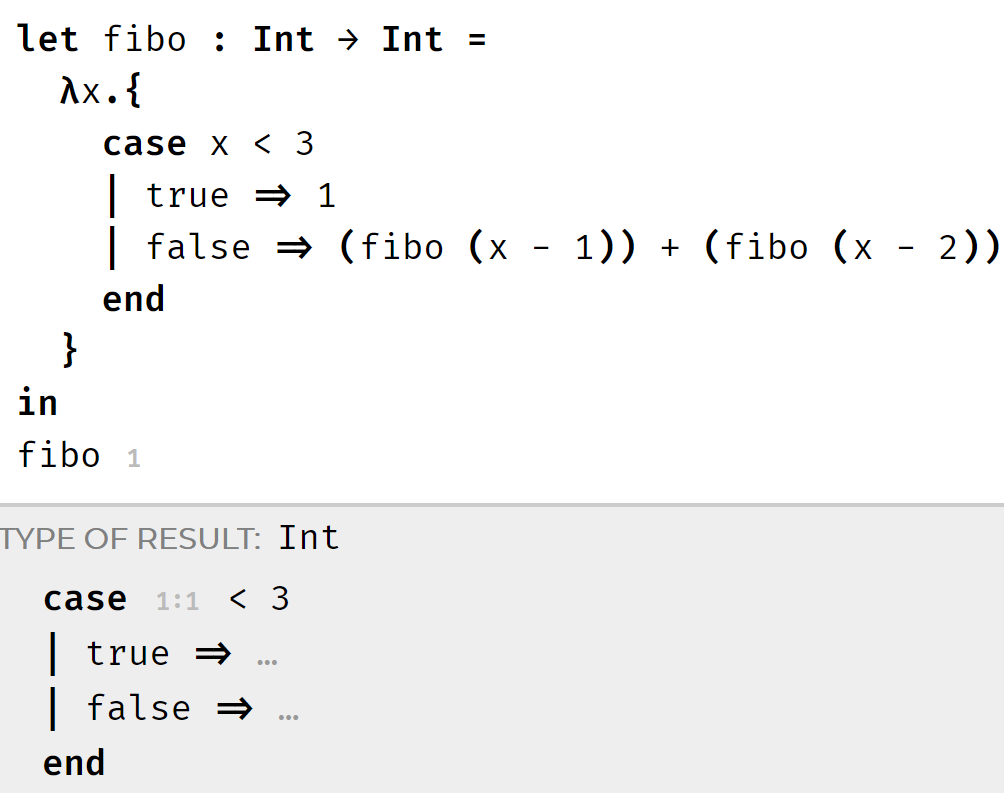
\includegraphics[width=0.8\textwidth]{img/pause_fibo.png}
      %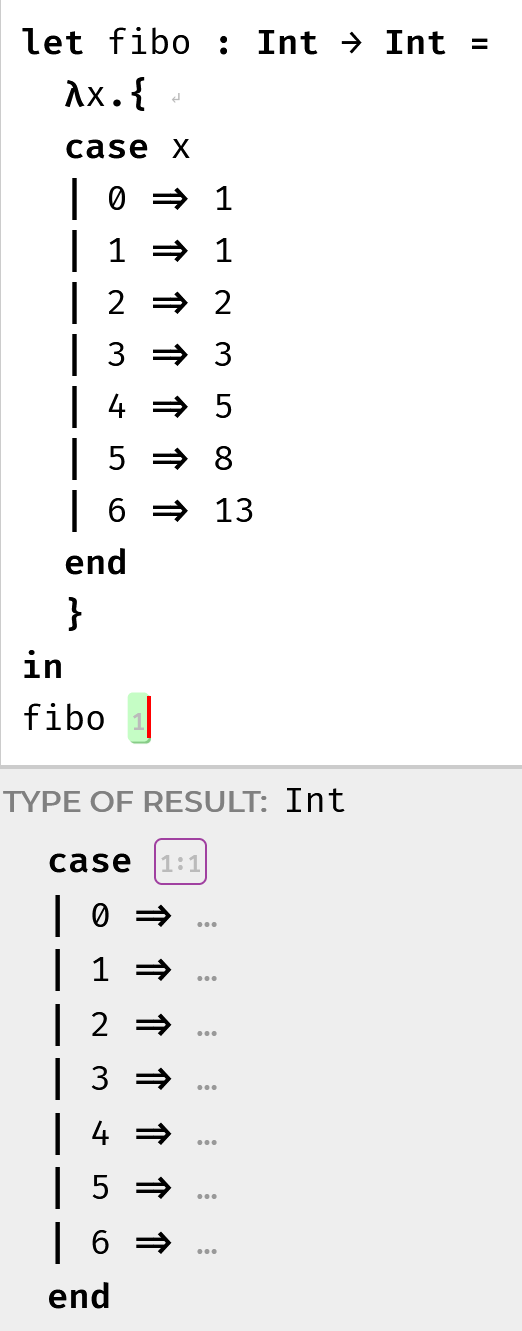
\includegraphics{img/pause_example.png}
      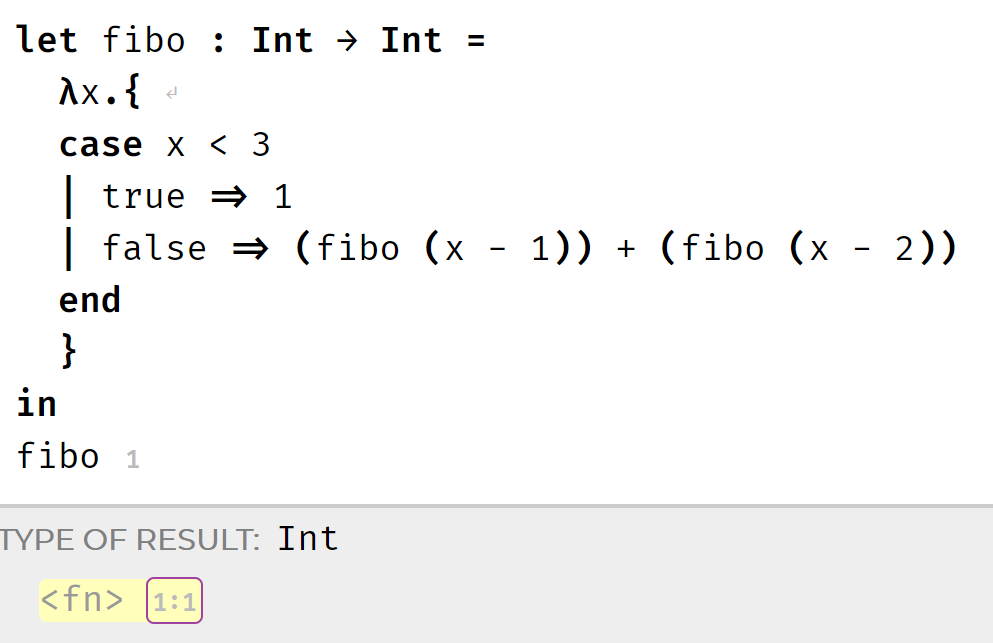
\includegraphics[width=0.8\textwidth]{img/pause_fibo2.png}
      \caption{Example of paused judgement}
      \label{fig:pause}
  \end{subfigure}
  \hfill
  \begin{subfigure}[b]{0.4\textwidth}
      \centering
      %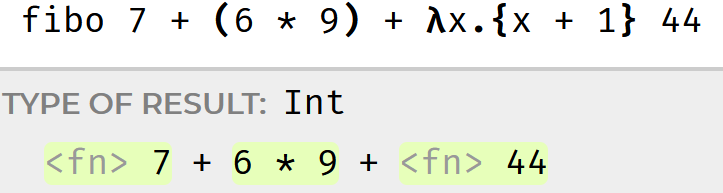
\includegraphics[width=\textwidth]{img/interactive.png}
      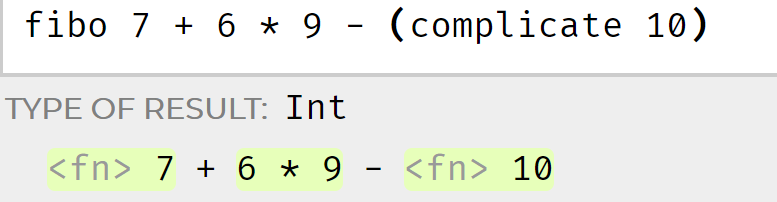
\includegraphics[width=\textwidth]{img/interactive1.png}
      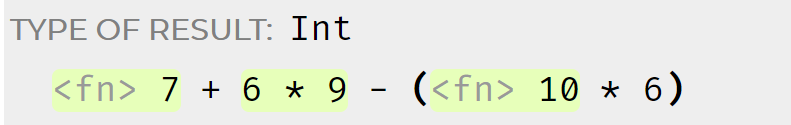
\includegraphics[width=\textwidth]{img/interactive2.png}
      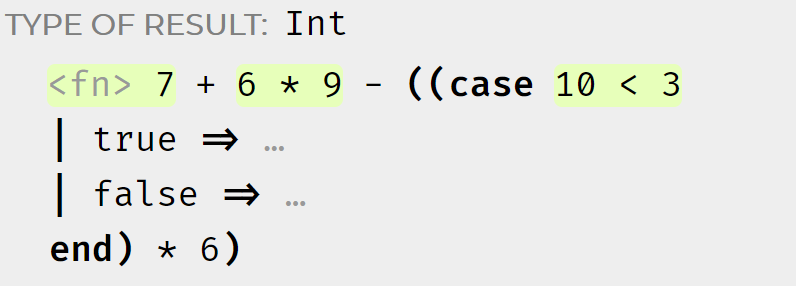
\includegraphics[width=\textwidth]{img/interacitve3.png}
      \caption{Example of multiple environment}
      \label{fig:multiple}
  \end{subfigure}
    \caption{Two programs in \Hazel}
    \label{fig:intro_example}
\end{figure}

% Findler et al.[citation] developed a stepper for DrScheme in their programming environment. Cong and Asai [citation] used the contextual dynamics to build a stepper, which takes subexpression out and plug in after evaluation. In this paper, we will use the similar strategy to develop the stepper. 

Figure \ref{fig:pause} is an example of expression with a hole. The evaluation result is a case expression with a hole as parameter. However, the origin expression is already simple enough and it is unnecessary to expand like that especially when there are many cases in the function. Therefore, we want to develop a stepper that can detect this situation so that it will pause until user requires it to step further. The result with yellow box is calculated by our stepper with pause judgement.

Figure \ref{fig:multiple} shows an expression with three parts. The left part is heavy since it takes many steps to evaluate. However, user might just want to debug the right complicated part. According to the regular dynamics, there should be only one way to step for any non-final programs. So, user has to click many times to reduce the left one in order to debug the right one. Our solution is to provide options for user to choose where to step. In the Figure \ref{fig:multiple}, the green boxes contain subexpressions that can be evaluated. In these three results, we always click the right box to evaluate. We can see how the multiple contexts work.

Our interactive stepper develops pausing judgement and a simple algorithm to decompose multiple evaluation contexts. Furthermore, it also has a webview so that user can click boxes to step expressions.

\parahead{Contributions} The contributions of this paper are: (1) a pausing judgement in section ~\ref{sec:pause}; (2) an algorithm to decompose multiple evaluation contexts in section ~\ref{sec:condy}.
%\section{Contextual Dynamics}
\label{sec:condy}


The structure of the stepper is shown in Figure \ref{fig:structure}. The expression is first decomposed into many independent evaluation contexts. Then, user may choose one of them to step. And the stepper will compose them into the final result then. For example, in Figure \ref{fig:multiple}, we have 3 evaluation contexts highlighted as green boxes. And when we click the second one, only the expression in second box is evaluated and composed into the whole expression.

\begin{figure}[htbp]
  \centering
  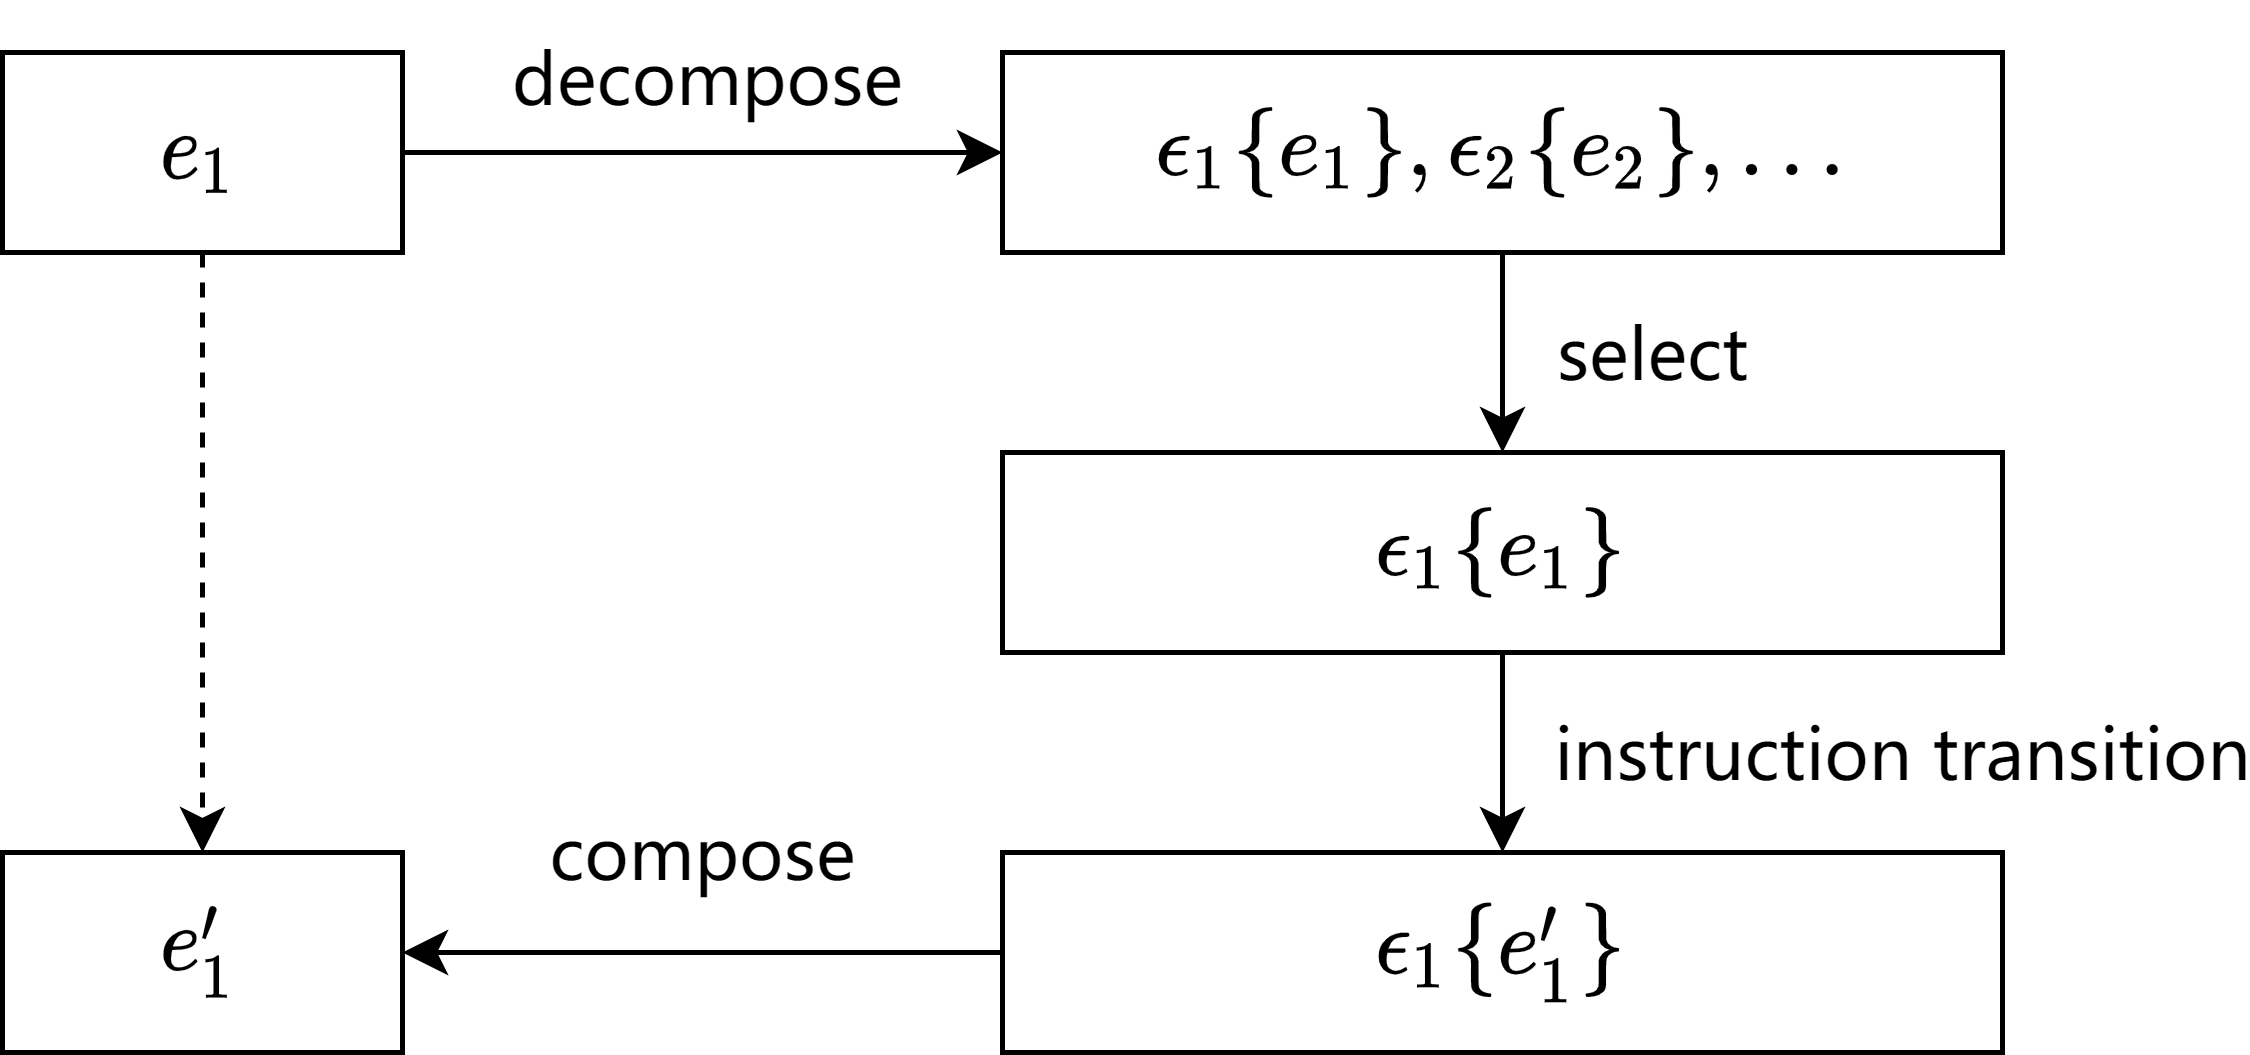
\includegraphics[width=0.5\textwidth]{img/struct.png}
  \caption{Structure of Stepper}
  \label{fig:structure}
\end{figure}

We now formally define the instruction transition judgement. We use $\htrans{e_1}{e_2}$ as instruction transition judgement. Figure \ref{fig:decompose} shows some of the transition judgements.

% As what Section \ref{sec:pause} discussed, in \Hazel, we have four types of expressions: $\mathtt{boxedvalue}$, $\mathtt{indet}$, $\mathtt{final}$, and $\mathtt{paused}$. The instruction transition can be implemented to provide the type of the expressions. Therefore, we can easily know whether an expression is final, paused or steppable.

Then, we formally define the evaluation context. Unlike the regular evaluation context, the decompose function will return a list of contexts. The decompose function is defined recursively. Figure \ref{fig:decompose} provides some of inference rules for decompose function.

\begin{figure}[htbp]
  \vspace{-3px} 
  \fbox{ $\htrans{e}{e'} $}~~\text{$e$ takes an instruction transition to $e'$}\hfill
  \begin{subequations}
  \label{eqns:instr_trans}
    \begin{mathpar}
        %\hfill
        \inferrule[]{\isFinal{e_2}
            }{
              \htrans{\hap{\lamfunc{x}{e_1}}{e_2}}{[e_2/x]e_1}
            }
        %\hfill
    \end{mathpar}
  \end{subequations}

$\arraycolsep=4pt\begin{array}{lll}
\text{EvalCtx}~~ \epsilon & ::= &
  \circ  ~\vert~
  \hap{\epsilon}{e} ~\vert~
  \hap{e}{\epsilon} ~\vert~
  \hhole{\epsilon} ~\vert~
  \epsilon + e ~\vert~
  e + \epsilon
\end{array}$

\fbox{ $\hdecom{e}{[\hcontext{\epsilon_1}{e_1}, \hcontext{\epsilon_2}{e_2}, \cdots]} $}~~\text{$e$ is decomposed into contexts $\hcontext{\epsilon_1}{e_1}$, $\hcontext{\epsilon_2}{e_2}$, $\cdots$}\hfill
  \begin{subequations}\label{eqns:decompose}
  \begin{mathpar}
      \hfill
      \inferrule[DFinal]{\isFinal{e}
          }{
            \hdecom{e}{[]}
          }\hfill
      \inferrule[DApFinal]{\isFinal{e_1} ~~\isFinal{e_2}}{\hdecom{\hap{e_1}{e_2}}{[\hcontext{\circ}{\hap{e_1}{e_2}}]}}
      \hfill\hfill
  \end{mathpar}
  \begin{mathpar}
    \hfill
      \inferrule[DAp]{\hdecom{e_1}{[\hcontext{\epsilon_1}{e_1'}, \cdots]}\\ \hdecom{e_2}{[\hcontext{\epsilon_2}{e_2'}, \cdots]}}{\hdecom{\hap{e_1}{e_2}}{[\hcontext{\hap{\epsilon_1}{e_2}}{e_1'}, \cdots, \hcontext{\hap{e_1}{\epsilon_2}}{e_2'}, \cdots]}}
      \hfill\hfill
  \end{mathpar}
  \begin{mathpar}
    \hfill
    \inferrule[DHole]{\hdecom{e}{[\hcontext{\epsilon}{e'}, \cdots]}}{\hdecom{\hhole{e}}{[\hcontext{\hhole{\epsilon}}{e'}]}}
      \hfill
      \inferrule[DAdd]{\hdecom{e_1}{[\hcontext{\epsilon_1}{e_1'}, \cdots]}\\ \hdecom{e_2}{[\hcontext{\epsilon_2}{e_2'}, \cdots]}}{\hdecom{(e_1 + e_2)}{[\hcontext{(\epsilon_1 + e_2)}{e_1'}, \cdots, \hcontext{(e_1 + \epsilon_2)}{e_2'}, \cdots]}}\hfill\hfill
  \end{mathpar}
\end{subequations}
\hrule
\caption{Insturction transition and decomposition}
  \label{fig:decompose}
  \vspace{-5px}
\end{figure}


For example, we have an expression $e_0 = 4 + 1 + (5 + 6)$. First, we know that $\hdecom{4 + 1}{[\hcontext{\circ}{4 + 1}]}$ and $\hdecom{5 + 6}{[\hcontext{\circ}{5 + 6}]}$. So, According to $\mathtt{DAdd}$ rule, we have,
$$
\hdecom{4 + 1 + (5 + 6)}{[\hcontext{(\circ + (5 + 6))}{4 + 1}, \hcontext{(4 + 1 + \circ)}{5 + 6}]}.
$$
User may choose second one so that the stepper will first evaluate $5 + 6$ and put result into mark. Hence, we get $4 + 1+ 11$ finally.
%\input{infalg}
%\section{Conclusion}

This paper develops an interactive stepper for \Hazel, hence, language environment with holes. It uses the Paused judgement to detect the unnecessary situation so that the stepper will stop over the paused expression. Also, we develop a simple algorithm for decomposition that can find all subexpressions which need to evaluate. We use the contextual dynamics to progress the expression for stepper. This result is useful for debugging or educational purpose.
\clearpage

\bibliographystyle{ACM-Reference-Format}
\bibliography{references,all.short,hazel_NSF}

\end{document}